\documentclass[12pt]{article}
%Gummi|065|=)
\usepackage{amsmath, amsfonts, amssymb}
\usepackage[margin=0.5in]{geometry}
\usepackage{xcolor}
\usepackage{graphicx}
%\usepackage{graphicx}
\newcommand{\off}[1]{}
\DeclareMathSizes{20}{30}{20}{18}
\newcommand{\myhrule}{}

\newcommand{\two }{\sqrt[3]{2}}
\newcommand{\four}{\sqrt[3]{4}}

\newcommand{\dash}{
\begin{tikzpicture}[scale=1]
\draw (0,0)--(19,0);
\end{tikzpicture}
}

\newcommand{\sq}[3]{
\node at (#1+0.5,#2+0.5) {#3};
\draw (#1+0,#2+0)--(#1+1,#2+0)--(#1+1,#2+1)--(#1+0,#2+1)--cycle;
}

\usepackage{tikz}

\title{\textbf{Proposal: Fermat Little Theorem}}
\author{John D Mangual}
\date{}
\begin{document}

\fontfamily{qag}\selectfont \fontsize{20}{25}\selectfont

\maketitle

\noindent In high school summer camp, we had a journal club and I read a proof of \textbf{F}ermat's \textbf{L}ittle \textbf{T}heorem:
$$\, a^p \equiv \; a  \; \pmod p $$
This theorem is important as soon as you need decimals. Let $a=10$ and $p = 7$:
$$ 10^7 \equiv 10 \pmod 7 $$
and clearly $7$ does not divide $10$, so we can just cancel:
$$ \hspace{1.7in} 10^6 = 1,000,000 \equiv 1 \pmod 7 $$
and we solved that problem without any long division.
$$ (10^6 - 1 ) \div 7 = 142,657$$
What is this good for?
\begin{itemize}
\item (statistical) \\ does this help us learn from real-world, empirical data?
\item (number theory)\\  does this help us solve other math problems?
\end{itemize}
I only know examples in the second category.  And that will have to be fine.


\newpage

\noindent We learned a ``proof" from a short article in Mathematics Magazine.  Consider the function:
$$ T: x \mapsto ax \pmod p $$ 
The orbits of $T^p$ are either cycles of order $p$ or a fixed point.  Except, we don't know what those are.  Instead we can draw on a square ($p=5$): \\\\
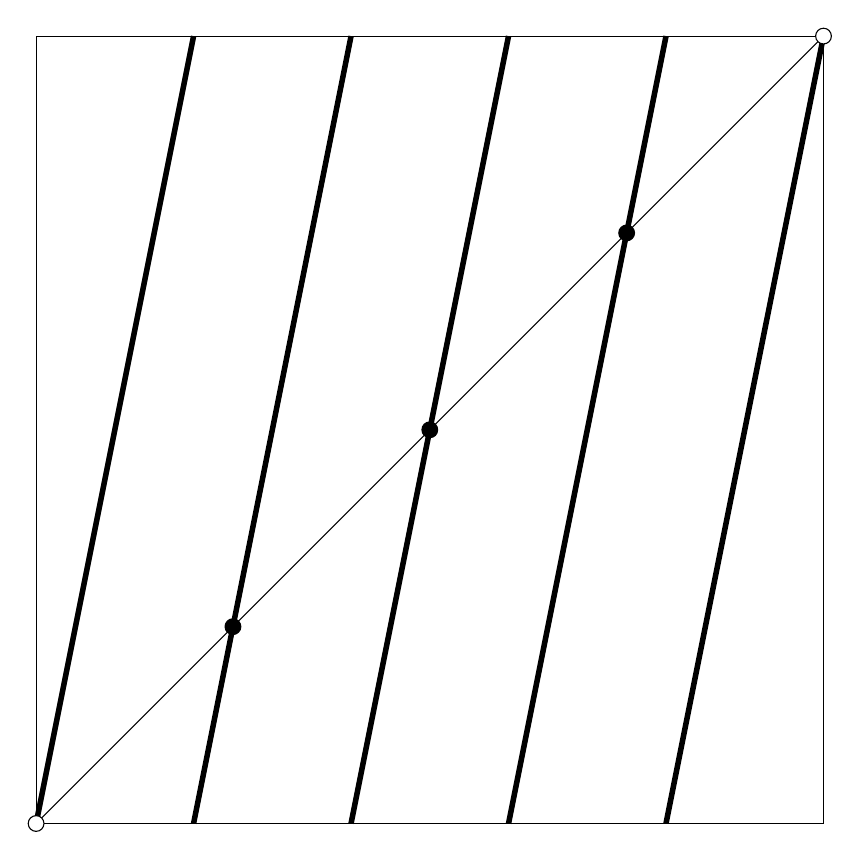
\begin{tikzpicture}[scale=10]
\draw (0,0)--(1,0)--(1,1)--(0,1)--cycle;
\draw[line width=2] (0/5,0)--(1/5,1);
\draw[line width=2] (1/5,0)--(2/5,1);
\draw[line width=2] (2/5,0)--(3/5,1);
\draw[line width=2] (3/5,0)--(4/5,1);
\draw[line width=2] (4/5,0)--(5/5,1);
\draw (0,0)--(1,1);
\draw[fill=white] (0/4,0/4) circle (0.01cm);
\draw[fill=black] (1/4,1/4) circle (0.01cm);
\draw[fill=black] (2/4,2/4) circle (0.01cm);
\draw[fill=black] (3/4,3/4) circle (0.01cm);
\draw[fill=white] (4/4,4/4) circle (0.01cm);
\end{tikzpicture} \\
There are three fixed points \begin{tikz} \draw[fill=black] (0/4,0/4) circle (0.25cm);\end{tikz}.  The two white circles \begin{tikz} \draw[fill=white] (0/4,0/4) circle (0.25cm);\end{tikz} count as half.   For a total of four, one less than our $p=5$. \\ \\
We can count the fixed points of $T^5: x \mapsto a^5 \, x$ and subtract off the fixed points of $T$.  This number should be divisible by $5$
$$ 5 \big| a^5 - a $$
and this is an instance of Fermat's Little Theorem.

\newpage

\noindent Can we get more mileage out of this proof.  Eventually we find out there is more:
$$ 15 \big| (a^5 - a)(a^3 - a) $$
and the Math Magazine proof has appeared several times from different people (in Math Magazine). \\ \\
I got a feeling there was something about our decimal system.  That if we chose an interesting enough $T$ (the dynamical system) we can get more interesting polynomial identities.

\newpage

\fontfamily{qag}\selectfont \fontsize{12}{10}\selectfont

\begin{thebibliography}{}

\item Iga, Kevin (2003), "\textbf{A Dynamical Systems Proof of Fermat's Little Theorem}", Mathematics Magazine, 76 (1): 48-51,


\end{thebibliography}



\end{document}